\graphicspath{{chapters/20/images}}
\chapter{Advanced methods}

\section{Adiabatic dynamics}
$n<3N$ reaction coordinates with generalized coordinates $q_\alpha$: the interest is in the free energy hypersurface $A(q_1, \dots, q_n)$.
Partition function:

$$Q(N, V, T) = C_N\int d^N\vec{p}d^N\vec{r}e^{-\beta\biggl[\sum\limits_{i=1}^N\frac{\vec{p}_i^2}{2m_i}+U(\vec{r}_1, \dots, \vec{r}_N)\biggr]}$$

Transformation to generalized coordinates $q_\alpha = f_\alpha(\vec{r}_1, \dots, \vec{r}_n)$ only for the configurational part, leaving momenta unchanged:

$$Q(N, V, T) = C_n\int d^N\vec{p}d^{3N}qe^{-\beta\biggl[\sum\limits_{i=1}^N\frac{\vec{p}_i^2}{2m_i} + \tilde{V}(q_1, \dots, q_{3N}, \beta)\biggr]}$$

Where:

$$\tilde{V}(q_1, \dots, q_{3N}, \beta) = \tilde{U}(q_1, \dots, q_{3N}) - kT\ln J(q_1, \dots, q_{3N})$$

$$\tilde{\mathcal{H}}(q, \vec{p}, \beta) = \sum\limits_{i=1}^N\frac{\vec{p}_i^2}{2m_i}+\tilde{V}(q_1, \dots, q_{3N}, \beta) = \sum\limits_{i=1}^N\frac{\vec{p}_i^2}{2m_i}+\tilde{U}(q_1, \dots, q_{3N})-kT\ln J(q_1, \dots, q_{3N})$$

This is not the original Hamiltonian but can be used as a Hamiltonian.
Renaming the momenta:

$$\tilde{H}(q, p, \beta) = \sum\limits_{\alpha=1}^{3N}\frac{p_\alpha^2}{2m'_\alpha}+ \tilde{V}(q_1, \dots, q_{3N}, \beta)$$

As in adiabatic free energy dynamics the first $n$ variables are thermostatted as a temperature $T_q\gg T$ with their masses increased so to adiabatically decouple them from the others.

	\subsection{TAMD}

	$$\tilde{H}(q, p, \beta) = \sum\limits_{\alpha=1}^{3N}\frac{p_\alpha^2}{2m'_\alpha} + \tilde{V}(q_1, \dots, q_{3N}, \beta)$$

	$$\dot{q}_\alpha = \frac{p_\alpha}{m'_\alpha}$$

	$$\dot{p}_\alpha = -\frac{\partial\tilde{V}}{\partial q_\alpha} - \frac{p_{\eta_1}}{Q_1}p_\alpha\quad \alpha= 1, \dots, n\qquad\dot{p}_\alpha = -\frac{\partial\tilde{V}}{\partial q_\alpha}-\frac{p_{\eta_e}}{Q_2}p_\alpha\quad \alpha = n_1, \dots, 3N$$

	$$\dot{p}_{\eta_1} = \sum\limits_{\alpha=1}^n\frac{p_\alpha^2}{2m'_\alpha}-nkT_q\qquad \dot{p}_{\epsilon_2} = \sum\limits_{\alpha=n+1}^{3N}\frac{p_\alpha^2}{2m'_\alpha}-(3N-n)kT$$

	It is possible to show that $A(q_1, \dots, q_n) = -kT_q\ln P_{adb}(q_1, \dots, q_n) + const$.

	\begin{figure}[H]
		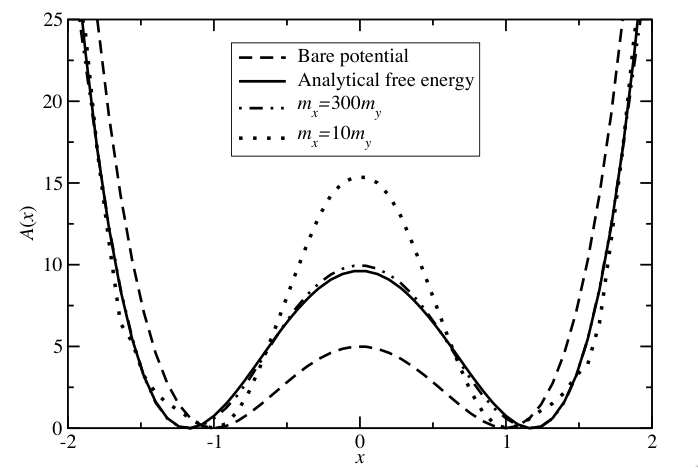
\includegraphics[width=\textwidth]{tamd}
		\caption{TAMD}
		\label{fig:tamd}
	\end{figure}

\section{Metadynamics}

$$P(s_1, \dots, s_n) = \biggl\langle\prod\limits_{\alpha=1}^n\delta(f_\alpha(\vec{r}_1, \dots, \vec{r}_N)-s_\alpha)\biggr\rangle$$

Replace the phase space average with a time average over a trajectory:

$$P(s_1, \dots, s_n) = \lim\limits_{\mathcal{T}\rightarrow\infty}\frac{1}{\mathcal{T}}\int_0^{\mathcal{T}} dt\prod\limits_{\alpha=1}^n\delta(f_\alpha(\vec{r}_1, \dots, \vec{r}_N)-s_\alpha)$$

However: $\delta(x-\alpha) = \lim\limits_{\sigma\rightarrow 0}\frac{1}{\sqrt{2\pi\sigma^2}}e^{-\frac{(x-\alpha)^2}{2\sigma^2}}$.

$$P(s_1, \dots, s_n) = \lim\limits_{\mathcal{T}\rightarrow\infty}\lim\limits_{\Delta s\rightarrow 0}\frac{1}{\mathcal{T}}\frac{1}{\sqrt{2\pi\Delta s^2}}\int_0^{\mathcal{T}}dt\prod\limits_{\alpha=1}^ne^{-\frac{(s_\alpha-f_\alpha(\vec{r}_1(t), \dots, \vec{r}_N(t)))^2}{2\Delta s^2}}$$

Bias potential:

$$U_G(\vec{r}_1, \dots, \vec{r}_N, t) = W\sum\limits_{t - \tau_G, 2\tau_G, \dots}e^{-\sum\limits_{\alpha=1}^n\frac{(f_\alpha(\vec{r})-f_\alpha(\vec{r}_G(t)))^2}{2\Delta s^2}}$$

\section{Transition path ensemble}

\begin{figure}[H]
	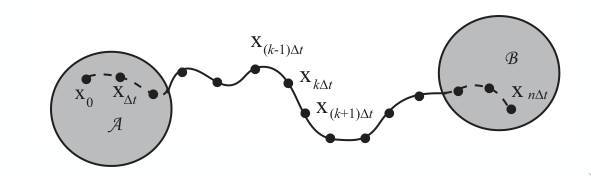
\includegraphics[width=\textwidth]{transition-path-ensemble}
	\caption{Transition path ensemble}
	\label{fig:transition-path-ensemble}
\end{figure}

$$x_{(k+1)\Delta t} = e^{iL_2\frac{\Delta t}{2}}e^{iL_1\Delta t}e^{iL_2\frac{\Delta t}{2}}x_{k\Delta t}\equiv\phi_{\Delta t}(x_{k\Delta t})$$

$$T(x_{(k+1)\Delta t}|x_{k\Delta t}) = \delta(x_{(k+1)\Delta t}-\phi_{\Delta t}(x_{k_{\Delta t}}))$$

Weight assigned to a single trajectory:

$$\mathcal{P}[X(\mathcal{T})] = f(x_0)\prod\limits_{k=0}^{n-1}T(x_{(k+1)\Delta t}|x_{k\Delta t})\qquad f(x_0) = \frac{e^{-\beta\mathcal{H}(x_0)}}{Q(N, V, T)}$$

$$\mathcal{P}[X(\mathcal{T})] = f(x_0)\prod\limits_{k=0}^{n-1}T(x_{(k+1)\Delta t}|x_{k\Delta t})$$

$$\mathcal{P}_{AB}[X(\mathcal{T})] = \frac{1}{\mathcal{F}_{AB}(\mathcal{T})}h_A(x_0)\mathcal{P}[X(\mathcal{T})]h_B(x_{n\Delta t})$$

$$F_{AB}(\mathcal{T}) = \int dx_0\cdots dx_{n\Delta t}h_a(x_0)\mathcal{P}[X(\mathcal{T})]h_B(x_{n\Delta t})$$

For deterministic molecular dynamics trajectories:

\begin{align*}
	\mathcal{F}_{AB}(\mathcal{T}) &= \int dx_0\cdots dx_{n\Delta t}h_A(x_0)f(x_0)\prod\limits_{k=1}^{n-1}\delta(x_{(k+1)\Delta t}-\phi_{\Delta t}(x_{k\Delta t}))h_B(x_{n\Delta t}) = \\
																&=\int dx_0h_A(x_0)f(x_0)h_B(x_{n\Delta t}(x_0))
\end{align*}

	\subsection{Transition path sampling}
	$\mathcal{R}_{AB}[X(\mathcal{T})|Y(\mathcal{T})]$ is the conditional probability to generate a trajectory $X(\mathcal{T})$ starting from $Y(\mathcal{T})$.
	Detailed balance condition:

	$$\mathcal{R}_{AB}[X(\mathcal{T})|Y(\mathcal{T})]\mathcal{P}_{AB}[Y(\mathcal{T})] = \mathcal{R}_{AB}[Y(\mathcal{T})|X(\mathcal{T})]\mathcal{P}_{AB}[X(\mathcal{T})]$$

	$$\mathcal{R}_{AB}[X(\mathcal{T})|Y(\mathcal{T})] = \Lambda_{AB}[X(\mathcal{T})|Y(\mathcal{T})]\mathcal{T}_{AB}[X(\mathcal{T})|Y(\mathcal{T})]$$

	$$\Lambda_{AB}[X(\mathcal{T})|Y(\mathcal{T})] = \min\biggl[1, \frac{\mathcal{T}_{AB}[Y(\mathcal{T})|X(\mathcal{T})]\mathcal{P}_{AB}[X(\mathcal{T})]}{\mathcal{T}_{AB}[X(\mathcal{T})|Y(\mathcal{T})]\mathcal{P}_{AB}[Y(\mathcal{T})]}\biggr]$$

	It is assumed that $Y[\mathcal{T}]$ is a proper trajectory from $A$ to $B$, hence $h_A(y_0) = 1$ and $h_b(y_{n\Delta t}) = 1$.

	$$\Lambda_{AB}[X(\mathcal{T})|Y(\mathcal{T})] = h_A(x_0)h_B(x_{n\Delta t})\min\biggl[1, \frac{\mathcal{T}_{AB}[Y(\mathcal{T})|X(\mathcal{T})]\mathcal{P}_{AB}[X(\mathcal{T})]}{\mathcal{T}_{AB}[X(\mathcal{T})|Y(\mathcal{T})]\mathcal{P}_{AB}[Y(\mathcal{T})]}\biggr]$$

	\begin{figure}[H]
		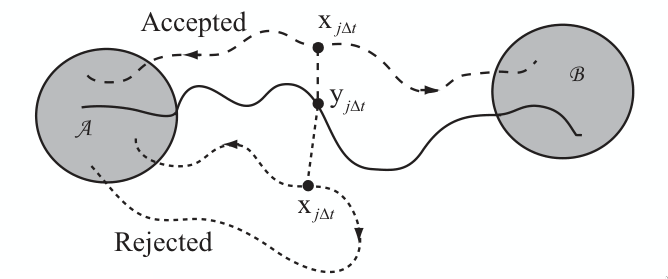
\includegraphics[width=\textwidth]{transition-path-sampling}
		\caption{Shooting move}
		\label{fig:shooting-move}
	\end{figure}

	$\tau(x_{j\Delta t}|y_{j\Delta t})$ is the rule to generate the shooting point.

	$$\mathcal{T}_{AB}[X(\mathcal{T})|Y(\mathcal{T})] = \tau(x_{j\Delta t}|y_{j\Delta t})\biggl[\prod\limits_{k=j}^{n-1}T(x_{(k+1)\Delta t}|x_{k\Delta t})\biggr]\biggl[\prod\limits_{k=1}^jT(x_{(k-1)\Delta t}|x_{k\Delta t})\biggr]$$

	\begin{align*}
		\Lambda_{AB}[X(\mathcal{T})|Y(\mathcal{T})] &= h_A(x_0)h_B(x_{n\Delta t})\min\biggl[1, \frac{\mathcal{T}_{AB}[Y(\mathcal{T})|X(\mathcal{T})]\mathcal{P}_{AB}[X(\mathcal{T})]}{\mathcal{T}_{AB}[X(\mathcal{T})|Y(\mathcal{T})]\mathcal{P}_{AB}[Y(\mathcal{T})]}\biggr] = \\
																								&= h_A(x_0)h_B(x_{n\Delta t})\min\biggl[1, \frac{f(x_0)}{f(y_0)}\biggl(\prod\limits_{k=0}^{n-1}\frac{T(x_{(k+1)\Delta t}|x_{k\Delta t})}{T(y_{(k+1)\Delta t}|y_k\Delta t)}\biggr)\biggl(\frac{\tau(y_{i\Delta t}|x_{j\Delta t})}{\tau(x_{j\Delta t}|y_{j\Delta t})}\cdot\\
																								&\qquad\qquad\qquad\qquad\qquad\qquad\cdot\prod\limits_{k=j}^{n-1}\frac{T(y_{(k+1)\Delta t}|y_{k\Delta t})}{T(x_{(k+1)\Delta t}|x_{k\Delta t})}\prod\limits_{k=0}^{j-1}\frac{T(y_{k\Delta t}|y_{(k+1)\Delta t})}{T(x_{k\Delta t}|x_{(k+1)\Delta t})}\biggr)\biggr] = \\
																								&=h_A(x_0)h_B(x_{n\Delta t})\min\biggl[1, \frac{f(x_0)}{f(y_0)}\frac{\tau(y_{j\Delta t}|x_{j\Delta t})}{\tau(x_{j\Delta t}|y_{j\Delta t})}\prod\limits_{k=0}^{j-1}\frac{T(x_{(k+1)\Delta t}|x_{k\Delta t})}{T(y_{(k+1)\Delta t}|y_{k\Delta t})}\frac{T(y_{k\Delta t}|y_{(k+1)\Delta t})}{T(x_{k\Delta t}|x_{(k+1)\Delta t})}\biggr]=\\
																								& = h_A(x_0)h_B(x_{n\Delta t})\min\biggl[1, \frac{f(x_0)}{f(y_0)}\frac{\tau(y_{j\Delta t}|x_{j\Delta t})}{\tau(x_{j\Delta t}|y_{j\Delta t})}\biggr]
	\end{align*}

	For a symmetric move $\tau(y_{j\Delta t}|x_{j\Delta t}) = \tau(x_{j\Delta t}|y_{j\Delta t})$:

	$$\Lambda_{AB}[X(\mathcal{T})|T(\mathcal{T})] = h_A(x_0)h_B(x_{n\Delta t})\min\biggl[1, \frac{f(x_0)}{f(y_0)}\biggr]$$

	Phase space displacement $\Delta = (0, \delta p)$

	\begin{enumerate}
		\item Choose an index $j$ randomly on the old trajectory $Y(\mathcal{T})$.
		\item Generate a random phase space displacement $\Delta$ in order to generate the new shooting point $x_{j\Delta t}$ from the old point $y_{j\Delta t}$.
		\item Integrate the equations of motion backwards in time from the shooting point to the initial condition $x_0$.
		\item If the initial condition $x_0$ is not in the phase space region $A$, reject the trial move.
		\item If $x_0\in A$ accept the move with probability $\min\biggl[1,\frac{f(x_0)}{f(y_0)}\biggr]$.
		\item Integrate the equations of motion forward in time to generate the final point $x_{n\Delta t}$.
		\item If $x_{n\Delta t}\in B$, accept the trial move, and reject it otherwise.
		\item If the path is rejected at steps $4, 5$ or $7$, then the old trajectory $Y(\mathcal{T})$ is counted again in the calculation of averages over the transition path ensemble
			Otherwise invert the momenta along the backward part of the path to yield a forward moving transition path $X(\mathcal{T})$ and replace the old trajectory $Y(\mathcal{T})$ by the new one $X(\mathcal{T})$
	\end{enumerate}

\section{The committor distribution}
The committor is the probability $p_B(\vec{r})$ that a trajectory initiated from a configruation $\vec{r}$ with velocities sampled from a Maxwell-Boltzmann distribution will arrive in state $B$ before state $A$.

\begin{figure}[H]
	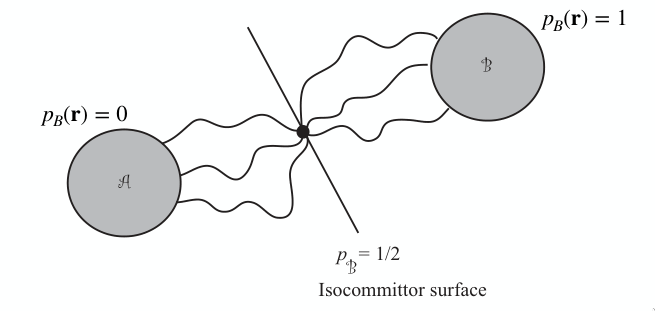
\includegraphics[width=\textwidth]{committor-distribution}
	\caption{The committor}
	\label{fig:committor-distribution}
\end{figure}

	\subsection{Histogram test}
	The committor $p_B(\vec{r})$ is an exact reaction coordinate for any system, but there is no analytic expression for it and obtaining it numerically is intractable
	The reaction coordinate $q(\vec{r})$ is good when the isosurfaces $q(\vec{r}) = const$ approximates the isosurfaces $p_B(\vec{r})= const$ of the committor.
	Committor distribution is the probability that $p_B(\vec{r}) = p$ when $q(\vec{r}) = q^{\ddagger}$, the value of $q(\vec{r})$ at a presumptive transition state.

	$$P(p) = \frac{C_N}{Q(N, V, T)}\int d^N\vec{p}\int_{q(\vec{r})=q^{\ddagger}}d^N\vec{r}e^{-\beta\mathcal{H}(\vec{r}, \vec{p})}\delta(p_B(\vec{r}_1, \dots, \vec{r}_N)-p)$$



	\subsection{Histogram test on $q_1(\vec{r}) = q^{\ddagger}$}

	\begin{enumerate}
		\item Fix the value $q_1(\vec{r}) = q^{\ddagger}$.
		\item $M$ configurations for the other variables $q_2^{(k)}(\vec{r}), \dots, q_{3N}^{(k)}(\vec{r})$.
		\item For each value of $k$, sample a set of initial velocities from a Maxwell-Boltzmann distribution.
		\item For each configuration $q^{\ddagger}, q_2^{(k)}(\vec{r}), \dots, q_{3N}^{(k)}(\vec{r})$, use each set of sampled velocities to initiate a trajectory the valu $1$ if it ends up in state $B$ and $0$ if it ends up in state $A$.
			Take the average for this value of $k$ and store it as $p^{(k)}$.
		\item Repeat for all of the configurations sampled in step $2$ to generate $p^{(1)}, \dots, p^{(M)}$.
		\item Plot a histogram for $p^{(1)}, \dots, p^{(M)}$.
	\end{enumerate}

	\begin{figure}[H]
		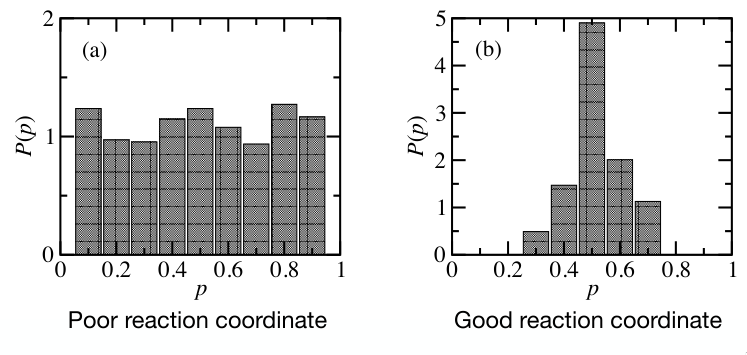
\includegraphics[width=\textwidth]{histogram-test}
		\caption{Histogram test example}
		\label{fig:histogram-test}
	\end{figure}
